% Copyright (C) 2016  Arvid Fahlström Myrman
%
% This program is free software; you can redistribute it and/or modify
% it under the terms of the GNU General Public License as published by
% the Free Software Foundation; either version 2 of the License, or
% (at your option) any later version.
%
% This program is distributed in the hope that it will be useful,
% but WITHOUT ANY WARRANTY; without even the implied warranty of
% MERCHANTABILITY or FITNESS FOR A PARTICULAR PURPOSE.  See the
% GNU General Public License for more details.
%
% You should have received a copy of the GNU General Public License along
% with this program; if not, write to the Free Software Foundation, Inc.,
% 51 Franklin Street, Fifth Floor, Boston, MA 02110-1301 USA.

% \begin{figure}
%   \centering
%   Sound + transcription + posteriorgrams
% 
%   \caption{\label{fig:postspec}Posteriorgram spectrum}
% \end{figure}

\chapter{Introduction}
\section{Background}
Automatic speech recognition (ASR) is generally framed as a supervised task, where both acoustic speech data and the corresponding transcription is available, and the problem is to develop a model that can mimic this mapping from speech to text.
However, developing such data is expensive, both in terms of time and money, as it involves painstakingly transcribing many hours of speech.
As a result, there is a notable lack of high-quality data for speech recognition for a majority of languages around the world.
An important question is thus whether it is possible to make use of untranscribed, or unlabelled, data to develop ASR for such low-resource languages.
Unsupervised learning in this manner may also provide insight into the linguistic structure of languages, or the language acquisition of infants.

We focus in particular on one aspect of unsupervised learning of speech, namely the discovery of phonetic classes, i.e.\ the basic speech sounds that make up all words in a language.
While supervised speech recognition makes use of prior knowledge regarding what sounds are present in a language, in unsupervised acquisition of speech this knowledge is unavailable to us.
This means that not only do we need to be able to discover what sounds make up each word in a recording without the use of a transcription---we need to discover what sounds are even available in the language to begin with, as not all languages use the same sounds, nor are the same sounds contrastive in all languages.
This is compounded by speaker variation, where there can be significant differences between the pronunciation of sounds by individual speakers, or even by the same speaker depending on e.g.\ the context of the sound.
This variation makes approaches such as naive clustering ineffective, as many of the discovered sounds are likely to be highly speaker-specific.

Unsupervised speech acquisition is an area of active research.
One source of such research is the Zero Resource Speech Challenge \parencite{versteegh2015zero}, which was developed with the goal of finding linguistic units (track 1) or longer recurring word-like fragments (track 2) in speech.
Models are to be trained using only speech data, voice activity information, and speaker identity information.
The main goal of the first track of the challenge is to find robust representations of speech frames where sounds belonging to the same phonetic category are more similar than sounds belonging to different categories; this is also the approach we will take in this work.

% Copyright (C) 2016  Arvid Fahlström Myrman
%
% This program is free software; you can redistribute it and/or modify
% it under the terms of the GNU General Public License as published by
% the Free Software Foundation; either version 2 of the License, or
% (at your option) any later version.
%
% This program is distributed in the hope that it will be useful,
% but WITHOUT ANY WARRANTY; without even the implied warranty of
% MERCHANTABILITY or FITNESS FOR A PARTICULAR PURPOSE.  See the
% GNU General Public License for more details.
%
% You should have received a copy of the GNU General Public License along
% with this program; if not, write to the Free Software Foundation, Inc.,
% 51 Franklin Street, Fifth Floor, Boston, MA 02110-1301 USA.

\chapter{Related work}
\label{ch:related-work}

This \namecref{ch:related-work} provides a brief overview of recent research into unsupervised acoustic modelling.
The approaches discussed here can broadly be divided into two categories: bottom-up approaches that infer the acoustic model directly from the speech frames, and top-down approaches that first segment the speech into syllable- or word-like units, and afterwards try break these units into smaller subword units.

\section{Bottom-up approaches}

As an individual speech frame only make up a fraction of a complete speech sound, it is natural to model and segment the speech using a model that can capture time dependencies, such as a hidden Markov model (HMM), rather than attempt to cluster the speech frames directly.
One issue with this approach, however, is that the number of possible states (i.e.\ subword units) is unknown a priori.

\textcite{varadarajan2008unsupervised} tackle this problem by first defining a one-state HMM, and then iteratively splitting and merging states as needed to account for the data according to a heuristic.
Training stops once the size of the HMM reaches a threshold.
After training, each state in the HMM can be thought to correspond to some allophone (context-dependent variant realisation) of a phoneme.
It should be noted, however, that in order to interpret a given state sequence as a single phoneme, \citeauthor{varadarajan2008unsupervised} train a separate model using labelled speech to perform this mapping.
The method is thus not fully unsupervised.

\textcite{lee2012nonparametric} take a fully probabilistic approach, defining a model that jointly performs segmentation and acoustic modelling.
An infinite mixture model of tri-state HMM-GMMs modelling subword units is defined using the Dirichlet process, and latent variables representing segment boundaries are introduced.
The data can be thought to be generated by repeatedly sampling an HMM to model a segment, sampling a path through the HMM, and for each state in the path sampling a feature vector from the corresponding GMM.
The probability of transitioning from one unit to another is thus not modelled.
Inference of the model is done using Gibbs sampling.

\textcite{siu2014unsupervised} use an HMM of a more classic form to model the data.
An initial transcription of the data in terms of state labels is first generated in an unsupervised manner using a segmental GMM (SGMM).
The HMM and transcription are then iteratively updated, maximising the probability of the model parameters given the transcription, and the transcription given the model parameters.
Note that the number of allowed states are here defined in advance.
$n$-gram statistics are then collected from the transcription and used for tasks such as unsupervised keyword discovery.

Diverging from previous approaches using temporal models, \textcite{chen2015parallel} perform standard clustering of speech frames using an infinite Gaussian mixture model.
After training, the speech frames are represented as posteriorgrams, which have been shown to be more speaker-invariant than other features such as MFCCs \parencite{zhang2010towards}.
Despite the simple approach, this turned out to be the overall best-performing model in the first track of the 2015 Zero Resource Speech Challenge \parencite{versteegh2016zero}.
\textcite{heck2016unsupervised} later further improved on the model by performing clustering in two stages, with an intermediate supervised dimensionality reduction step using the clusters derived from the first clustering step as target classes.

\textcite{synnaeve2016temporal} use a siamese network to create an embedding where speech frames close to each other are considered to belong to the same subword unit, while distant speech frames are said to differ.
A siamese network is a feedforward neural network that takes two inputs and adjusts its parameters to either maximise or minimise the similarity of the corresponding outputs \parencite{bromley1994signature}.

\section{Top-down approaches}
\todo[inline]{remove information already included in the introduction}

Top-down approaches start by first finding pairs of longer word-like segments using unsupervised term discovery (UTD).
This information provides constraints that can be use to find speech frame representations that are more stable within a given subword unit.
The rationale is that while at the frame level the same speech sound can seem quite different between different speakers or even different realisations of the sound by the same speaker, patterns over a longer duration of time are easier to identify; this idea is illustrated in \textcite{jansen2013weak}.

The UTD systems used in this context are generally based on the segmental dynamic time warping (S-DTW) developed by \textcite{park2008unsupervised}.
S-DTW works by repeatedly performing DTW on two audio streams while constraining the maximum amount of warping allowed, each time changing the starting point of the DTW in both streams.
This yields a set of alignments, from which the stretches of lowest average dissimilarity in each alignment can be extracted.
Unfortunately, this approach is inherently $O(n^2)$ in time.
To remedy this, \textcite{jansen2011efficient} introduced an approximate version that uses binary approximations of the feature vectors to perform the calculations in $O(n \log n)$ time using sparse similarity matrices; this system also serves as the baseline for the second track of the Zero Resource Speech Challenge \parencite{versteegh2015zero}.

\textcite{jansen2011towards} describe a method for finding subword units, assuming that clusters corresponding to words, each cluster containing multiple examples of that word in the form of audio, are given.
For each word, an HMM is trained on all the corresponding examples, the number of states in the model being set to a number proportional to the average duration of the word.
The states from each HMM are then collected and clustered based on the similarity of their distributions, forming clusters that hopefully correspond to subword units.

\textcite{jansen2013weak} take somewhat of an inverse approach, starting by clustering the whole data on a frame level, with the assumption that each cluster will tend to correspond to some speaker- or context-dependent subword unit.
They then look at pairs of word-like segments known to be of the same type and calculate how often clusters tend to co-occurr.
The clusters are then partitioned so that clusters that co-occurr often are placed in the same partition.

\textcite{synnaeve2014phonetics} introduce a neural network known referred to as the ABnet, based on siamese networks \parencite{bromley1994signature}.
The network takes a pair of speech frames as input, and adjusts its parameters so that the outputs are collinear if the inputs are known to correspond to the same subword unit, and orthogonal otherwise, using a cosine-based loss function.
\textcite{thiolliere2015hybrid} made use of this approach in the Zero Resource Speech Challenge, also incorporating unsupervised term discovery so as to make the whole process unsupervised, yielding competitive results \parencite{versteegh2016zero}.
\textcite{zeghidour2016deep} experiment with supplying the ABnet with scattering spectrum features instead of filter bank features, showing that with the right features, a shallow architecture may outperform a deep architecture, especially when the amount of available data is low.

\textcite{kamper2015unsupervised} use an autoencoder-like structure, where a neural network is trained to ``reconstruct'' a frame given another frame known to be of the same type.
\textcite{renshaw2015comparison} used this architecture in the Zero Resource Speech Challenge, albeit with a deeper decoder.

\section{This thesis}
\todo[inline]{make description more application agnostic?}

Two of the most successful approaches so far are the clustering approach of \textcite{chen2015parallel} and the siamese network approach of \textcite{thiolliere2015hybrid}.
We pose the question of whether it is possible to combine the two approaches by first clustering the data in an unsupervised manner using a probabilistic model, and then improving the resulting posteriorgrams using speech fragment information.
This way we are able to take advantage of both the whole unlabelled data set, and the smaller set of discovered fragments.

Many probabilistic models, such as Gaussian mixture models and hidden Markov models, have a concept of latent states or classes.
We pose the problem of improving posteriorgrams from such a model as one of merging, or partitioning, these classes.
By first training the model in a fully unsupervised manner, it learns classes that can generally be assumed to be highly speaker-specific.
We can then use weak supervision to merge these classes, yielding representations that are more speaker invariant.

A partitioning of classes can be viewed as a surjection from the original set of classes to a class set of lower cardinality, but finding this surjection is a discrete problem which is difficult to optimise for.
However, a benefit of posteriorgrams is that the probability of an output class can be described as a simple sum of the probabilities of the classes that map to the class in question.
This means that the surjection can be approximated using a continuous linear model which can be optimised through standard gradient descent.
A linear model also has the added benefit of being more interpretable than deep networks such as that of \textcite{thiolliere2015hybrid}.
While the approach of partitioning posteriorgrams is very reminiscent of \textcite{jansen2013weak}, the major difference is that in place of direct clustering of classes, we are instead trying to maximise the similarity/dissimilarity between pairs of speech fragments, which only indirectly results in a partitioning of the classes.


\section{This thesis}

\begin{figure}
  \centering
  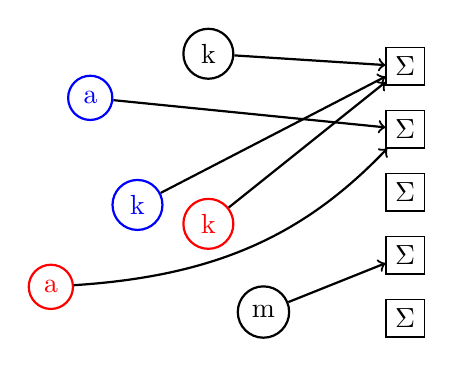
\begin{tikzpicture}[outpos/.style={draw,rectangle},inpos/.style={draw,circle,thick},
    arr/.style={->,thick},yscale=0.8]
    \node[outpos] at (0,0) {$\Sigma$};
    \node[outpos] (out3) at (0,1) {$\Sigma$};
    \node[outpos] at (0,2) {$\Sigma$};
    \node[outpos] (out2) at (0,3) {$\Sigma$};
    \node[outpos] (out1) at (0,4) {$\Sigma$};
    
    \node[inpos,blue] (a1) at (-4, 3.5) {a};
    \node[inpos,red] (a2) at (-4.5, 0.5) {a};
    \node[inpos,blue] (k1) at (-3.4, 1.8) {k};
    \node[inpos,red] (k2) at (-2.5, 1.5) {k};
    \node[inpos] (k3) at (-2.5, 4.2) {k};
    \node[inpos] (m1) at (-1.8, 0.1) {m};
    
    \draw (a1) edge[arr] (out2) (a2) edge[arr,bend right=24] (out2)
          (k1) edge[arr] (out1) (k2) edge[arr] (out1) (k3) edge[arr] (out1)
	  (m1) edge[arr] (out3);
  \end{tikzpicture}

  \caption{\label{fig:mapping}An example of merging speaker-specific (coloured) clusters by mapping them to (a subset of) the available outputs.
  As we represent the input as a probability vector, each output is a simple sum of the input probabilities.}
\end{figure}

We take inspiration from two of the most successful approaches so far: the clustering approach of \textcite{chen2015parallel} and the siamese network approach of \textcite{thiolliere2015hybrid}, described above.
We pose the question of whether it is possible to combine the two approaches.
One way to do this is to first cluster the whole data set in a fully unsupervised manner, discovering latent classes from the data such that similar data points belong to the same latent class.
By extracting a latent representation of the data from the clustering model, we can then improve on this representation using speech fragment information.
This way we are able to take advantage of both the complete unlabelled data set, and the smaller set of discovered fragments.

For this work we consider in particular probabilistic models such as Gaussian mixture models and hidden Markov models.
These models express class membership in terms of probabilities, giving the posterior probability of each data point belonging to one of the latent classes.
By representing each data point as a vector of these posterior probabilities, called a posteriorgram, the task of improving this representation can be framed as one of merging, or partitioning, the latent classes appropriately.
Latent classes discovered through unsupervised training will generally be high speaker-specific.
However, by merging the classes using weak supervision in the form of speech fragment pairs, we can construct classes that are more speaker invariant.

A partitioning of classes can be viewed as finding a function which maps the original set of classes to a class set of lower cardinality, but finding this function is a discrete problem which is difficult to optimise for.
However, a benefit of posteriorgrams is that the probability of an output class can be described as a simple sum of the probabilities of the input classes that map to the output in question, as illustrated in \cref{fig:mapping}.
This means that the mapping function can be approximated using a continuous linear model which can be optimised through standard gradient descent.
A linear model also has the added benefit of being more interpretable than deep networks such as that of \textcite{thiolliere2015hybrid}.
While the approach of partitioning posteriorgrams is very reminiscent of \textcite{jansen2013weak}, the major difference is that in place of direct clustering of classes, we are instead trying to maximise the similarity/dissimilarity between pairs of speech fragments, which only indirectly results in a partitioning of the classes.

\begin{figure}
  \centering
  \begin{tikzpicture}
    %\begin{axis}[enlargelimits=false,axis on top,width=8cm,height=4cm,ylabel={Frequency (\si\Hz)},xlabel={Time (\si\s)}]
    %\end{axis}

% speaker 1
% s3102b 146.518752 147.111647 questions
%   146.518752  122 ng
%   146.596735  122 k
%   146.624258  122 w
%   146.693066  122 ah
%   146.760727  122 s; *
%   146.816920  122 ch
%   147.021050  122 en
%   147.111647  122 z

% speaker 2
% s2302a 106.778375 107.628939 questions
%   106.778375  122 ng
%   106.883302  122 k
%   106.921215  122 w
%   106.985553  122 eh
%   107.098375  122 s ; *
%   107.168375  122 ch
%   107.246360  122 ah
%   107.348375  122 n
%   107.628939  122 z
    \begin{groupplot}[group style={group size=2 by 3, horizontal sep=2cm, vertical sep=0.4cm},
      enlargelimits=false,width=6.5cm,height=5.7cm,axis on top,xtick=\empty]
      \nextgroupplot[ylabel={Frequency (\si\Hz)},title={Female speaker}]
      \addplot graphics[xmin=146.52,xmax=147.11,ymin=0,ymax=3125] {data/spectrum-speaker-1-crop.pdf};
      \coordinate (kw1t) at (axis cs:146.59,\pgfkeysvalueof{/pgfplots/ymax});
      \coordinate (we1t) at (axis cs:146.62,\pgfkeysvalueof{/pgfplots/ymax});
      \coordinate (es1t) at (axis cs:146.69,\pgfkeysvalueof{/pgfplots/ymax});
      \coordinate (sc1t) at (axis cs:146.76,\pgfkeysvalueof{/pgfplots/ymax});
      \coordinate (cu1t) at (axis cs:146.82,\pgfkeysvalueof{/pgfplots/ymax});
      \coordinate (un1t) at (axis cs:147.02,\pgfkeysvalueof{/pgfplots/ymax});

      \nextgroupplot[title={Male speaker}]
      \addplot graphics[xmin=106.78,xmax=107.63,ymin=0,ymax=3125] {data/spectrum-speaker-2-crop.pdf};
      \coordinate (kw2t) at (axis cs:106.88,\pgfkeysvalueof{/pgfplots/ymax});
      \coordinate (we2t) at (axis cs:106.92,\pgfkeysvalueof{/pgfplots/ymax});
      \coordinate (es2t) at (axis cs:106.99,\pgfkeysvalueof{/pgfplots/ymax});
      \coordinate (sc2t) at (axis cs:107.10,\pgfkeysvalueof{/pgfplots/ymax});
      \coordinate (cu2t) at (axis cs:107.17,\pgfkeysvalueof{/pgfplots/ymax});
      \coordinate (un2t) at (axis cs:107.35,\pgfkeysvalueof{/pgfplots/ymax});
      
      \nextgroupplot[ylabel={GMM component}]
      \addplot graphics[xmin=146.52,xmax=147.11,ymin=1,ymax=1024] {data/gmm-posteriorgrams-speaker-1-crop.pdf};
      
      \nextgroupplot
      \addplot graphics[xmin=106.78,xmax=107.63,ymin=1,ymax=1024] {data/gmm-posteriorgrams-speaker-2-crop.pdf};
      
      \nextgroupplot[ylabel={Model output},xlabel={Time}]
      \addplot graphics[xmin=146.52,xmax=147.11,ymin=1,ymax=33] {data/reduced-posteriorgrams-speaker-1-crop.pdf};
      \coordinate (kw1b) at (axis cs:146.59,\pgfkeysvalueof{/pgfplots/ymin});
      \coordinate (we1b) at (axis cs:146.62,\pgfkeysvalueof{/pgfplots/ymin});
      \coordinate (es1b) at (axis cs:146.69,\pgfkeysvalueof{/pgfplots/ymin});
      \coordinate (sc1b) at (axis cs:146.76,\pgfkeysvalueof{/pgfplots/ymin});
      \coordinate (cu1b) at (axis cs:146.82,\pgfkeysvalueof{/pgfplots/ymin});
      \coordinate (un1b) at (axis cs:147.02,\pgfkeysvalueof{/pgfplots/ymin});
      
      \nextgroupplot[xlabel={Time}]
      \addplot graphics[xmin=106.78,xmax=107.63,ymin=1,ymax=33] {data/reduced-posteriorgrams-speaker-2-crop.pdf};
      \coordinate (kw2b) at (axis cs:106.88,\pgfkeysvalueof{/pgfplots/ymin});
      \coordinate (we2b) at (axis cs:106.92,\pgfkeysvalueof{/pgfplots/ymin});
      \coordinate (es2b) at (axis cs:106.99,\pgfkeysvalueof{/pgfplots/ymin});
      \coordinate (sc2b) at (axis cs:107.10,\pgfkeysvalueof{/pgfplots/ymin});
      \coordinate (cu2b) at (axis cs:107.17,\pgfkeysvalueof{/pgfplots/ymin});
      \coordinate (un2b) at (axis cs:107.35,\pgfkeysvalueof{/pgfplots/ymin});

  \end{groupplot}
  \draw [thin,white] (kw1t) -- (kw1b);
  \draw [thin,white] (we1t) -- (we1b);
  \draw [thin,white] (es1t) -- (es1b);
  \draw [thin,white] (sc1t) -- (sc1b);
  \draw [thin,white] (cu1t) -- (cu1b);
  \draw [thin,white] (un1t) -- (un1b);
  
  \draw [thin,white] (kw2t) -- (kw2b);
  \draw [thin,white] (we2t) -- (we2b);
  \draw [thin,white] (es2t) -- (es2b);
  \draw [thin,white] (sc2t) -- (sc2b);
  \draw [thin,white] (cu2t) -- (cu2b);
  \draw [thin,white] (un2t) -- (un2b);
  \end{tikzpicture}

  \caption{\label{fig:model-output}Example of using the proposed model to process utterances of the word ``question'' from two different speakers.
  First the energy spectrum is calculated for each speech frame (top).
  After preprocessing the spectrum is then fed to a Gaussian mixture model from which posterior probabilities for each latent class is extracted (middle).
  Last, the probability vectors from the GMM are reduced in size using the proposed model (bottom).
  The white crosses mark the most probable class state for each frame.
  The white vertical lines mark boundaries between speech sounds.
  The example is meant to be illustrative and does not represent the overall performance of the model.}
\end{figure}

Using such a linear model, we hope to use speech fragment information to improve on posteriorgrams obtained from an unsupervised probabilistic model.
In particular we hope to use the model to construct more speaker-invariant posteriorgrams which can be used to discriminate between different linguistic units in a robust manner.
An example of using the model can be seen in \cref{fig:model-output}; the model takes high-dimensional posteriorgrams describing a probability distribution over latent variables (classes) from a Gaussian mixture model, and outputs low-dimensional posteriorgrams which are more speaker invariant.
We evaluate the model using the minimal-pair ABX task used for evaluation in the first track of the Zero Resource Speech Challenge.
